\documentclass{article}
\pdfpagewidth=8.5in
\pdfpageheight=11in

\usepackage{POBRreport}
% Use the postscript times font!
\usepackage{times}
\usepackage{soul}
\usepackage{url}
\usepackage{xcolor}
\usepackage{polski}
\usepackage[polish]{babel}
\usepackage[utf8]{inputenc}
\usepackage[T1]{fontenc}
\usepackage[utf8]{luainputenc}
\usepackage[hidelinks]{hyperref}
\usepackage[utf8]{inputenc}
\usepackage{caption}
\usepackage{indentfirst}
\usepackage{graphicx}
\usepackage{amsmath}
\usepackage{booktabs}
\usepackage{subfig}
\usepackage{float}
\usepackage{pgfplots}
\usepackage{listings}
\usepackage{color}
\usepackage{siunitx}
\usepackage{graphicx}
\usepackage{tikz}

\renewcommand{\labelitemii}{$\circ$}
\urlstyle{same}

\title{Przetwarzanie Cyfrowe Obrazów \\ Wykrywanie logo restauracji Burger King}

\author{
Jakub Sikora
\affiliations
nr albumu: 283418\\
\emails
jakub.sikora2.stud@pw.edu.pl
}

\newcommand{\bk}{
    Burger King
}
\newcommand{\todo}[1]{\textcolor{blue}{\textbf{TO DO:} #1}}

\begin{document}

\maketitle

\section{Treść zadania}
\label{sec:cel-projektu}
Celem projektu jest praktyczne zapoznanie się studentów z cyfrowymi metodami przetwarzania, analizy i rozpoznawania obrazów. 

Dla obrazów zawierających logo restauracji \bk należy dobrać, zaimplementować i przetestować odpowiednie procedury wstępnego przetworzenia, segmentacji, wyznaczania cech oraz identyfikacji obrazów cyfrowych. Powstały w wyniku projektu program powinien poprawnie rozpoznawać wybrane obiekty dla reprezentatywnego zestawu obrazów wejściowych. W trakcie projektu należy przetestować wybrane algorytmy i ocenić ich praktyczną przydatność. Wnioski powstałe w trakcie projektu muszą zostać przedstawione w formie pisemnego sprawozdania. Zaliczenie projektu dokonywane jest na podstawie pokazu działania zrealizowanego programu oraz sprawozdania. Sprawozdanie ma zawierać wyszczególnienie wybranych i zaimplementowanych algorytmów oraz wnioski powstałe w trakcie implementacji i testowania programu.

Jako dane wejściowe muszą być wykorzystane: zdjęcia w postaci papierowej - wykonane własnoręcznie lub wybrane np. z książek i czasopism, które należy zeskanować; lub zdjęcia w postaci cyfrowej - uzyskane za pomocą aparatu cyfrowego. Danych wejściowych nie mogą stanowić obrazy uzyskane bezpośrednio cyfrowo tzn. np. z programów typu MS Paint, Corel Draw itp. Ponadto w projekcie nie można wykorzystywać funkcji bibliotecznych do przetwarzania, analizy oraz rozpoznawania obrazów.


\section{Logo restauracji \bk}
\label{sec:logo-bk}
Przedstawione na rysunku \ref{fig:bklogo} logo restauracji \bk składa się z~czterech części:
\begin{itemize}
    \item czerwonego napisu \bk,
    \item żółtej bułki od burgera podzielonej na pół,
    \item niebieskiej paska okalającego napis,
    \item białego okrągłego tła.
\end{itemize}

\begin{figure}[tb]
    \centering
    
\includegraphics[width=0.4\columnwidth]{./figures/bklogo.pdf}
    \caption{Logo restauracji \bk~\cite{WikipediaEN:bklogo}}
    \label{fig:bklogo}
\end{figure}

Każda z~części ma swoją stałą, rozróżnialną barwę, co pozwala ją w~pełni rozróżnić od innych elementów. Poszczególne elementy praktycznie nienachodzą na siebie, nie licząc kawałka czerwonego napisu zachodzącego na fragment niebieskiej obwódki. Logo jest wpisane w~okrąg, dzięki czemu dobrze skaluje się w~przestrzeni.

Typowo, logo \bk można znaleźć na elewacjach budynków tej restauracji, na znakach przydrożnych oraz wewnątrz samej restauracji. Co więcej, logo może być przedstawione z~wewnętrznym podświetleniem lub bez niego. Powoduje to bardzo zmienne warunki oświetleniowe znaku, co mimo prostego zestawu barw, czyni z~niego ciekawy obiekt do automatycznego wykrywania.


\section{Akwizycja obrazu}
\label{sec:akwizycja-obrazu}
\todo{zrobić zdjęcia jak już będzie można wychodzić, opisać aparat jakim to robiłem}

\section{Zarys algorytmu przetwarzania}
\label{sec:algorytm}
W~zaproponowanym algorytmie wykrywania logo \bk, można wydzielić pięć odrębnych faz przetwarzania. Poszczególne fazy zostały zaprezentowane za pomocą schematu blokowego na rysunku~\ref{fig:algorithm-overview}.

\begin{figure}[h]
    \centering
    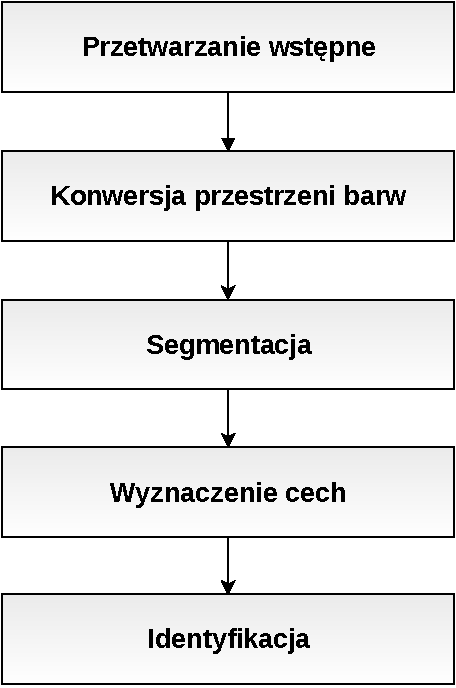
\includegraphics[width=0.6\columnwidth]{figures/algorithmOverview.pdf}
    \caption{Ogólny schemat blokowy algorytmu wykrywania logo \bk}
    \label{fig:algorithm-overview}
\end{figure}

W~pierwszej kolejności obraz zostanie przepuszczony przez moduł przetwarzania wstępnego. Jego zadaniem jest poprawa jakości obrazu oraz ujednolicenie jego rozmiaru.
Następnie obraz zostanie skonwertowany do odpowiedniej przestrzeni barw, tak aby móc przeprowadzić proces segmentacji obrazu. Dla każdego wykrytego segmentu, wyznaczone zostanie dla niego zestaw cech, na podstawie których przeprowadzony zostanie etap identyfikacji.

\subsection{Szczegóły implementacyjne}
Cały algorytm wykrywania został zaimplementowany przy pomocy języka C++. Program korzysta ze specjalnie przygotowanych klas i~narzędzi, realizujących podstawowe algorytmy przetwarzania obrazu, zagregowanych w~pakiecie \texttt{POBR}. Akwizycja obrazu, jego wyświetlanie, zapisywanie oraz przechowywanie w~pamięci zostało zrealizowane za pomocą biblioteki OpenCV~\cite{opencv}. Działanie aplikacji sterowane jest za pomocą szeregu parametrów, które są wczytywane z~pliku konfiguracyjnego w~formacie YAML.

\section{Przetwarzanie wstępne}
\label{sec:preprocessing}
Pierwszym krokiem algorytmu wykrywania logo \bk, jest przetwarzanie wstępne. Celem przetwarzania wstępnego jest zmniejszenie rzeczywistego rozmiaru obrazu, względna poprawa jego jakości oraz usunięcie zakłóceń.

\subsection{Skalowanie obrazu}
Celem skalowania obrazu jest stworzenie nowego obrazu o~zmienionym rozmiarze, wykorzystując do tego obraz oryginalny. W~przypadku projektowanego systemu, obraz analizowany jest poddawany skalowaniu aby zmniejszyć jego rzeczywisty rozmiar, celem uproszczenia dalszych obliczeń.

Do zmiany rozdzielczości obrazu cyfrowego zwykle wykorzystuje się metody interpolacji. Algorytmy tego typu można podzielić na algorytmy nieadaptacyjne oraz adaptacyjne. Pierwsza grupa dokonuje interpolacji w~ustalony z~góry sposób, niezależnie od zawartości przetwarzanego obrazu. Algorytmy adaptacyjne zmieniają sposób przetwarzania pikseli, biorąc pod uwagę cechy aktualnie przetwarzanego fragmentu. Adaptacja pozwala na zwiększenie jakości wizualnej, zwiększając przy tym koszt obliczeniowy~\cite{swierczynski2008podwyzszanie}.

W~ramach projektu przeanalizowałem działanie trzech algorytmów nieadaptacyjnych: 
\begin{itemize}
    \item interpolacja najbliższym sąsiadem,
    \item interpolacja dwuliniowa,
    \item interpolacja dwukubiczna.
\end{itemize}

Wymienione algorytmy różnią się ilością punktów branych pod uwagę podczas obliczania jasności piksela w~obrazie wynikowym. W~pierwszym kroku każdego algorytmu oblicza się w~którym miejscu w~obrazie wejściowym znajduje się rozpatrywany punkt obrazu wyjściowego. Dokonuje się tego poprzez obliczenie współczynników skalowania, zgodnie z~wzorami~\ref{eqn:wsp-skalowania-x}~i~\ref{eqn:wsp-skalowania-y}.

\begin{equation}
    \label{eqn:wsp-skalowania-x}
    r_{x} = \frac{\mathrm{width}_{input}}{\mathrm{width}_{output}}
\end{equation}

\begin{equation}
    \label{eqn:wsp-skalowania-y}
    r_{y} = \frac{\mathrm{height}_{input}}{\mathrm{height}_{output}}
\end{equation}

Na podstawie współczynników $r_{x}, r_{y}$ dla piksela $(i, j)$ obrazu wyjściowego oblicza się pozycję~$(x, y)$ w~obrazie wejściowym, wykorzystując zależność \ref{eqn:skalowanie}.

\begin{equation}
    \label{eqn:skalowanie}
    \begin{array}{ll}
        x = i \cdot r_{x} & y = j \cdot r_{y}
    \end{array} 
\end{equation}

\subsubsection{Interpolacja najbliższym sąsiadem}
Interpolacja metodą najbliższego sąsiada jest najprostszą metodą zmiany rozmiaru obrazu cyfrowego. Jest to metoda wymagająca najmniejszej mocy obliczeniowej i~jest jedyną metodą nie powodującą rozmycia obrazu wynikowego. W~przetwarzaniu obrazów jest najczęściej wykorzystywana do zmiany rozmiaru zdjęć zawierających kody kreskowe lub zrzutów ekranu aplikacji okienkowych.

Algorytm interpolacji najbliższym sąsiadem działa w~sposób przedstawiony na rysunku~\ref{fig:nn-example}. Dla każdej obliczonej pary $(x,y)$ odpowiadającej pikselowi $(i, j)$ w~obrazie wyjściowym, wybierany jest rzeczywisty piksel $(\hat{x}, \hat{y})$ obrazu wejściowego, którego odległość punktu docelowego jest najmniejsza (czyli jest najbliższym sąsiadem obliczonego piksela).

\begin{figure}[h]
    \centering
    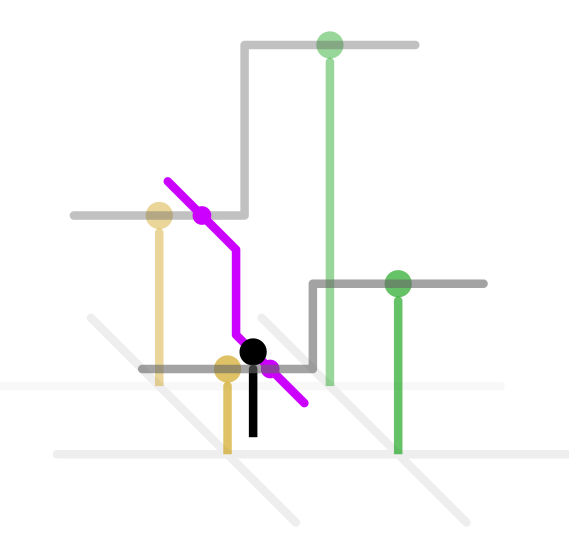
\includegraphics[width=0.6\columnwidth]{figures/nearestneighbour.png}
    \caption{Wybór najbliższego sąsiada w~algorytmie interpolacji~\cite{WikipediaEN:bicubicimg}}
    \label{fig:nn-example}
\end{figure}

W~stworzonym rozwiązaniu, algorytm interpolacji dwuliniowej jest implementowany przez  obiekty klasy \texttt{POBR::NearestNeighbourInterpolationResizer}. Wyniki działania tego algorytmu zostały przedstawione na rysunku~\ref{fig:nearestneighbour-result}. 

\begin{figure}[h]
    \centering
    \subfloat[25x25px]{{
\includegraphics[scale=2.6]{figures/25x25/nn.png}}}
    \qquad
    \subfloat[50x50px]{{
\includegraphics[scale=1.3]{./figures/50x50.jpg} }}%
    \qquad
    \subfloat[100x100px]{{
\includegraphics[scale=0.65]{./figures/100x100/nn.png} }}
    \caption{Efekt działania algorytmu interpolacji najbliższym sąsiadem na przykładzie zmniejszania logo \bk z~rozmiaru 50x50px do 25x25px oraz zwiększania do rozmiaru 100x100px}
    \label{fig:nearestneighbour-result}
\end{figure}

Obrazy przetworzone za pomocą algorytmu interpolacją najbliższego sąsiada cechują się blokowatością. Brak rozmycia powoduje że obraz traci naturalny wygląd. Jest to jednak metoda najszybsza, warta rozważenia w~zadaniach automatycznego wykrywania obiektów.

\subsubsection{Interpolacja dwuliniowa}
Algorytm interpolacji dwuliniowej jest algorytmem nieadaptacyjnym, nieco bardziej zaawansowanym niż pokrewny algorytm najbliższego sąsiada. Wartość każdego piksela obrazu wynikowego jest obliczana na podstawie czterech sąsiednich punktów obrazu wejściowego~\cite{algorytmy:bilinear}.

Na podstawie informacji o~docelowym punkcie, wybiera się cztery najbliższe punkty $F_{0,0}, F_{0,1}, F_{1,0}, F_{1,1}$, tak jak to przedstawiono na~\ref{fig:bilinear-result} (żółtym kolorem zaznaczono punkt obliczony z~wzorów~\ref{eqn:skalowanie}). 

\begin{figure}[h]
    \centering
    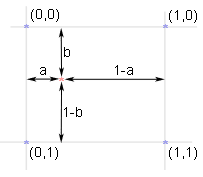
\includegraphics[width=0.6\columnwidth]{figures/bi2.png}
    \caption{Dobór sąsiednich punktów w~algorytmie interpolacji dwuliniowej~\cite{algorytmy:bilinear}}
    \label{fig:bilinear-example}
\end{figure}

Następnie trzykrotnie przeprowadza się interpolację pomiędzy punktami, najpierw dwa razy w~kierunku poziomym pomiędzy $F_{0,0}$~i~$F_{1,0}$ oraz $F_{0,1}$~i~$F_{1,1}$ i~ostatni raz pomiędzy wynikami poprzednich interpolacji, zgodnie ze wzorem~\ref{eqn:interpolacja}. Proces ten należy powtórzyć dla każdej składowej koloru z~osobna~\cite{algorytmy:bilinear}.

\begin{equation}
    \label{eqn:interpolacja}
    \begin{array}{l}
        F_{a,0} = (1-a) \cdot F_{0,0} + a \cdot F_{1,0} \\
        F_{a,1} = (1-a) \cdot F_{0,1} + a \cdot F_{1,1} \\
        F_{a,b} = (1-b) \cdot F_{a,0} + b \cdot F_{0,1} \\
    \end{array} 
\end{equation}

W~stworzonym rozwiązaniu, algorytm interpolacji dwuliniowej jest implementowany przez  obiekty klasy \texttt{POBR::BilinearInterpolationResizer}. Wyniki działania tego algorytmu zostały przedstawione na rysunku~\ref{fig:bilinear-result}.

\begin{figure}[h]
    \centering
    \subfloat[25x25px]{{
\includegraphics[scale=2.6]{figures/25x25/bl.png}}}
    \qquad
    \subfloat[50x50px]{{
\includegraphics[scale=1.3]{./figures/50x50.jpg} }}
    \qquad
    \subfloat[100x100px]{{
\includegraphics[scale=0.65]{./figures/100x100/bl.png} }}
    \caption{Efekt działania algorytmu interpolacji dwuliniowej na przykładzie zmniejszania logo \bk z~rozmiaru 50x50px do 25x25px oraz zwiększania do rozmiaru 100x100px}
    \label{fig:bilinear-result}
\end{figure}

Algorytm interpolacji dwuliniowej jest zdecydowanie bardziej skomplikowanym algorytmem przetwarzania. W~wyniku jego działania, obraz wyjściowy jest rozmyty, co jednak pozwala na zachowanie naturalnego wyglądu obrazu. Mimo brania pod uwagę czterech pikseli, metoda ta niewiele mocniej obciąża procesor. 

\subsubsection{Interpolacja dwukubiczna}
Interpolacja dwukubiczna jest najczęściej wykorzystywanym algorytmem zmiany rozmiaru obrazu, szczególnie w~system gdzie prędkość przetwarzania nie jest najważniejszym kryterium. Zamiast czterech najbliższych punktów, algorytm bierze pod uwagę szesnaście najbliższych punktowi docelowemu pikseli. Obrazy przetworzone przez algorytm dwukubiczny mają znacznie gładsze krawędzie oraz pozbawione są widocznych artefaktów.

\begin{figure}[h]
    \centering
    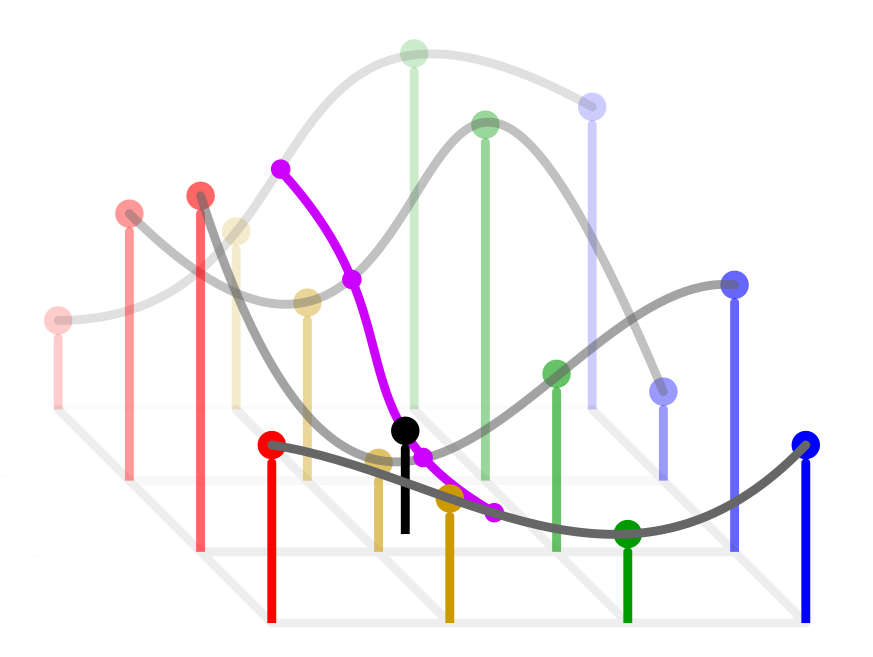
\includegraphics[width=\columnwidth]{figures/bicubic.png}
    \caption{Zasada działania algorytmu interpolacji dwukubicznej~\cite{WikipediaEN:bicubicimg}}
    \label{fig:bicubic-example}
\end{figure}

Poglądowo, zasada działania algorytmu została przedstawiona na rysunku~\ref{fig:bicubic-example}. Do wyznaczenia wartości jasności danego piksela, algorytm bierze pod uwagę szesnaście pikseli w~bezpośrednim otoczeniu wyznaczonej pozycji $(x,y)$ piksela. Podobnie jak w~algorytmie dwuliniowym, w~pierwszej kolejności dokonywana jest interpolacja w~osi poziomej, tym razem jednak czterokrotnie, dla czterech rzędów pikseli. Funkcje jasności są lokalnie interpolowane wielomianem trzeciego stopnia. Następnym krokiem algorytmu jest ponowna interpolacja, tym razem w~osi pionowej. Operację należy powtórzyć dla każdej zmiennej składowej obrazu.

Przygotowany system udostępnia klasę realizującą algorytm interpolacji dwukubicznej o~nazwie \texttt{POBR::BicubicInterpolationResizer}. Na rysunku~\ref{fig:bicubic-result} zostały przedstawione wyniki działania algorytmu w~zadaniu zmniejszania oraz zwiększania oryginalnego obrazka.

\begin{figure}[h]
    \centering
    \subfloat[25x25px]{{
\includegraphics[scale=2.6]{figures/25x25/bc.png}}}
    \qquad
    \subfloat[50x50px]{{
\includegraphics[scale=1.3]{./figures/50x50.jpg} }}%
    \qquad
    \subfloat[100x100px]{{
\includegraphics[scale=0.65]{./figures/100x100/bc.png} }}%
    \caption{Efekt działania algorytmu interpolacji dwukubicznej na przykładzie zmniejszania logo \bk z~rozmiaru 50x50px do 25x25px oraz zwiększania do rozmiaru 100x100px}
    \label{fig:bicubic-result}
\end{figure}

Obrazki otrzymane w~wyniku działania algorytmu są najprzyjemniejsze dla oka. Krawędzie są naturalnie rozmyte. Jedyną wadą tego algorytmu skalowania jest czas jego trwania. Algorytm ten zdecydowanie nie nadaje się do przetwarzania obrazów w~czasie rzeczywistym.

W~celu wyboru algorytmu zmiany rozmiaru obrazka do projektowanego systemu wykrywania, przeprowadziłem eksperyment porównawczy. Pojedynczy obrazek o~wielkości 200x200px został powiększony przez każdy z~trzech algorytmów do wielu różnych rozmiarów. Następnie porównano wyniki oraz czasy przetwarzania. 

\begin{figure}[h]
    \centering
    \begin{tikzpicture}
        \pgfplotsset{%
            y tick label style={/pgf/number format/.cd,fixed,precision=4},
            x tick label style={/pgf/number format/1000 sep=\,},
        }  
        \begin{axis}[
            grid=minor,
            xmode=log,
            ymode=log,
            xlabel={rozmiar [px]},
            ylabel={czas przetwarzania [s]},
            ytick={0.0001, 0.001, 0.01, 0.1, 1, 10, 100},
            log ticks with fixed point
        ]
            \addplot[mark=*, red, semithick] table {
                50 0.000305484
                100 0.00173367
                200 0.00479529
                400 0.0186251
                800 0.102972
                1600 0.348162
                3200 1.26685
                6400 4.18572
            };
            \addplot[mark=*, blue, semithick] table {
                50 0.00056756
                100 0.00179102
                200 0.00344637
                400 0.0138544
                800 0.0935612
                1600 0.345652
                3200 1.55231
                6400 4.94573
            };
            \addplot[mark=*, green, semithick] table {
                50 0.0104428 
                100 0.0473796 
                200 0.0828924 
                400 0.245594 
                800 0.750946 
                1600 2.64254 
                3200 11.2324 
                6400 50.3934 
            };
        \end{axis}
    \end{tikzpicture}
    \caption{Porównanie czasu zmiany obrazka 200x200px do docelowego rozmiaru w~zależności od długości boku kwadratowego obrazka}
    \label{fig:resizing-time}
\end{figure}

Zgodnie z~oczekiwaniami, najlepsze rezultaty zostały osiągnięte przez algorytm interpolacji dwukubicznej. Nawet przy dziesięciokrotnym powiększeniu, obrazek nadal wyglądał naturalnie i~zdecydowanie lepiej od pozostałych.  

Na wykresie~\ref{fig:resizing-time} przedstawiono zależność czasu przetwarzania od rozmiaru obrazka. Algorytmy najbliższego sąsiada oraz interpolacji dwuliniowej działają w~porównywalnym czasie, natomiast algorytm dwukubiczny znacznie odstaje od pozostałych dwóch, działając średnio o~rząd wielkości dłużej.

Na podstawie wykonanego eksperymentu, zdecydowałem się na wybór algorytmu interpolacji dwukubicznej. Krótki czas przetwarzania nie jest szczególnie oczekiwaną cechą od projektowanego systemu oraz algorytm będzie stosowany do zmniejszania obrazków a~nie do ich znacznego powiększania, dlatego też z~wszystkich trzech przedstawionych rozwiązań, algorytm dwukubiczny jest najlepszy.

\subsection{Filtracja}
Po zmianie rozmiaru zdjęcia, kolejnym krokiem była jego filtracja. Celem filtracji jest pozbycie się zakłóceń w~obrazie. W~ramach projektu zaimplementowałem i~przetestowałem następujące filtry:
\begin{itemize}
    \item splotowe,
    \begin{itemize}
        \item dolnoprzepustowe,
        \item górnoprzepustowe,
        \item gaussowskie,
    \end{itemize}
    \item statystyczne,
    \begin{itemize}
        \item minimum,
        \item maksimum,
        \item medianowy.
    \end{itemize}
\end{itemize}

Wartość funkcji jasności nowego piksela przefiltrowanego oblicza się na podstawie wartości funkcji jasności pikseli sąsiadujących z~nim. W~wyniku działania algorytmu filtracyjnego musi powstać nowa kopia obrazu. 

Ciekawym zagadnieniem w~filtracji tego typu jest zachowanie algorytmu na brzegach obrazu, gdzie nie każdy piksel ma pełne sąsiedztwo. Algorytm może przyjąć jedną z~wielu strategii ekstrapolacji obrazu. W~OpenCV~\cite{opencv} zaimplementowano następujące strategie:
\begin{itemize}
    \item \emph{BORDER\_{}REPLICATE} -- algorytm powiela piksele brzegowe tyle razy, ile wynosi połowa okna przetwarzania filtru,
    \item \emph{BORDER\_{}REFLECT} -- algorytm dokonuje lustrzanego odbicia pikseli znajdujących się przy granicy obrazka,
    \item \emph{BORDER\_{}WRAP} -- algorytm zawija obraz i~korzysta z~pikseli znajdujących się po drugiej stronie obrazka,
    \item \emph{BORDER\_{}CONSTANT} -- algorytm wypełnia brakujące piksele pewną podaną stałą wartością.
\end{itemize}

W~przypadku postawionego problemu, gdzie poszukiwane logo zazwyczaj jest sporych rozmiarów oraz składa się z~wielu komponentów, zdecydowałem się na porzucenie przedstawionych strategii i~zaimplementowanie własnej, polegającej na pomijaniu pikseli brzegowych.

\subsubsection{Implementacja filtrów w języku C++}
Każdy z~zaimplementowanych filtrów opisany jest przez rozmiar swojego okna. Język C++ pozwala na definiowanie własnych typów parametryzowanych, przy użyciu szablonów. Dzięki temu, stosując technikę metaprogramowania, można zaimplementować parametryzowane funkcję filtrujące, w~których rozmiar okna jest argumentem typu. Takie podejście pozwala na znaczne przyspieszenie kodu, gdyż pozwala na rozwinięcie pętli filtru a~co za tym idzie, uniknięcie kosztownych instrukcji skoku procesora. 

Mimo niewątpliwych zalet metaprogramowania, umyślnie zdecydowałem się na implementację filtru w~sposób klasyczny z~wykorzystaniem pętli. Każda zmiana rozmiaru filtru wiązałaby się z~ponowną rekompilacją programu, natomiast gdy rozmiar filtru podany jest jako parametr wczytywany z~pliku, pozwala to na przetestowanie większej liczby rozwiązań. 

\subsubsection{Wykorzystanie w projekcie}
Metodą prób i~błędów, dobrałem zestaw filtrów, którymi traktowany jest każdy obraz przed rozpoczęciem segmentacji. 

W~pierwszej kolejności z~obrazu należy odfiltrować zakłócenia. Do tego wykorzystany może zostać filtr dolnoprzepustowy, medianowy lub gaussowski. Po przetestowaniu każdego z nich, ostatecznie zdecydowałem się na filtr gaussowski o~rozmiarze okna 5x5 pikseli oraz jednakowym odchyleniu standardowym w~każdej osi $\sigma_{\mathrm{x}} = \sigma_{\mathrm{y}} = 2{,}0$. Zastosowanie delikatnego filtru pozwala na odfiltrowanie zakłóceń, zostawiając przy tym kontury elementów poszukiwanego znaku. 

W~celu podkreślenia różnic pomiędzy kolorowymi fragmentami, w~następnym kroku dokonałem filtracji górnoprzepustowej filtrem o~nieznormalizowanym oknie 3x3:

$$
\begin{bmatrix}
    -0{,}5 & -0{,}5 & -0{,}5 \\
    -0{,}5 &  5{,}0 & -0{,}5 \\
    -0{,}5 & -0{,}5 & -0{,}5 
\end{bmatrix}
$$

Rezultaty filtracji zostały przedstawione na rysunku~\ref{fig:filters-result}. Na ostatnim rysunku nadal dość dobrze można rozróżnić poszczególne elementy znaku graficznego.

Celem przedstawionego procesu filtracji było odfiltrowanie zakłóceń przy zachowaniu widocznych granic pomiędzy poszczególnymi kolorami znaku graficznego. Dzięki temu, w~dalszych krokach możliwym będzie przeprowadzenie segmentacji opartej o~różnice w~jasności pikseli. Innym podejściem mogłoby być przeprowadzanie  takiej filtracji, której celem byłoby wyeksponowanie krawędzi w~obrazie, tak aby móc przeprowadzić segmentację konturową. Filtry realizujące tego typu operacje nazywane są filtrami konturowymi. Przykładowym filtrem tego typu jest filtr Sobela oraz filtr Prewitta.

\begin{figure}[H]
    \centering
    \subfloat[Przed filtracją]{{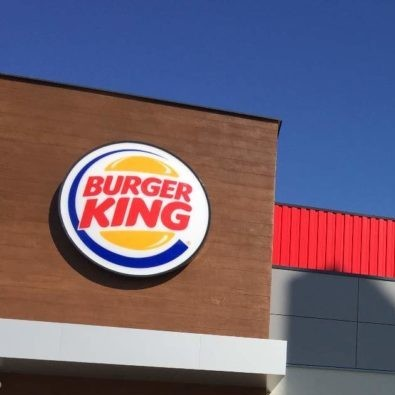
\includegraphics[scale=2.0]{./figures/filters/bk1.jpg}}}
    \\
    \subfloat[Po filtracji gaussowskiej]{{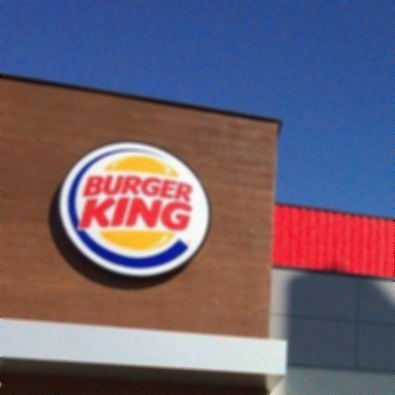
\includegraphics[scale=0.48]{./figures/filters/gauss.jpg}}}%
    \\
    \subfloat[Po filtracji górnoprzepustowej]{{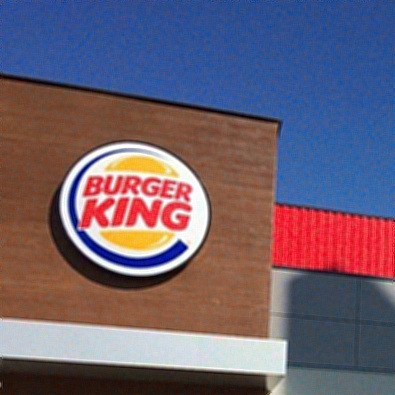
\includegraphics[scale=0.48]{./figures/filters/highpass.jpg} }}%
    \caption{Efekt działania filtrów w programie}
    \label{fig:filters-result}
\end{figure}

\section{Konwersja przestrzeni barw}
\label{sec:przestrzenie}
Po przetwarzaniu wstępnym obrazu, kolejnym krokiem algorytmu wykrywania logo \bk była konwersja przestrzeni barw z~RGB do przestrzeni~HSV.

\subsection{Przestrzeń RGB}
Najbardziej znanym modelem przestrzeni barw jest model opisywany współrzędnymi RGB. Nazwa współrzędnych pochodzi od pierwszych liter nazw barw podstawowych: (\textbf{R})~czerwonej, (\textbf{G})~zielonej oraz (\textbf{B})~niebieskiej. Model ten bazuje na właściwościach ludzkiego oka. Wrażenie widzenia dowolnej barwy można uzyskać poprzez zmieszanie trzech wiązek światła \cite{jankowski1990elementy}.

Model RGB jest domyślnie wykorzystywany w~informatyce do przechowywania plików graficznych. Wykorzystywana w~rozwiązaniu biblioteka OpenCV, również bazuje na tym modelu, odwracając kolejność kolorów. Zamiast jako pierwszą przechowywać informację o kolorze czerwonym, pierwsza przechowywana informacja mówi o~kolorze niebieskim, tak jak zostało to przedstawione na rysunku~\ref{fig:bgr}. Tak odwróconą przestrzeń nazywa się przestrzenią BGR~\cite{opencv}.

\begin{figure}[h]
    \centering
    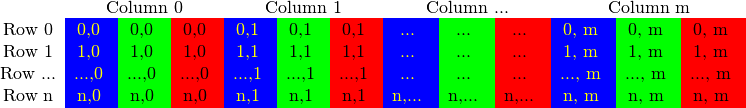
\includegraphics[width=\columnwidth]{./figures/opencv-matrix-bgr.png}
    \caption{Sposób reprezentacji obrazu w~przestrzeni BGR, wykorzystywanej w~OpenCV~\cite{opencv}}
    \label{fig:bgr}
\end{figure}

\subsection{Przestrzeń HSV}
Model HSV czerpie swoją nazwę od pierwszych liter angielskich nazw składowych: \textbf{H} - hue (barwa), \textbf{S} - saturation (nasycenie), \textbf{V} - value (wartość). Model ten znacznie różni się od poprzednio omawianego modelu. W~RGB, wszystkie trzy zmienne niosą jednocześnie informację na temat chrominancji (kolorze) i~luminancji (jasności) punktu. W~modelu HSV, tylko jedna składowa \textbf{V} niesie informację o~jasności piksela a~pozostałe dwie zmienne \textbf{H}~i~\textbf{S}~przechowują informację o~chrominancji piksela. Taki sposób reprezentacji znacznie ułatwia wykrywanie na zdjęciu obiektów o~danej barwie lecz o~różnym oświetleniu. Typowo, przestrzeń HSV przedstawia się za pomocą stożka, zaprezentowanego na rysunku~\ref{fig:hsv}.

\begin{figure}[h]
    \centering
    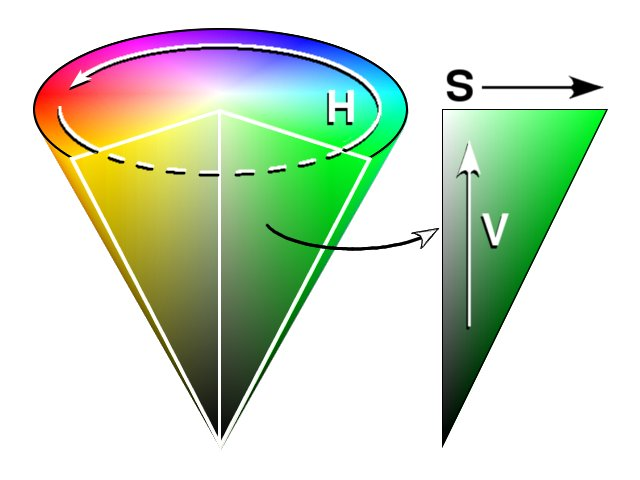
\includegraphics[width=0.6\columnwidth]{./figures/HSV_cone.jpg}
    \caption{Stożek przestrzeni barw HSV~\cite{WikipediaPL:hsvCone}}
    \label{fig:hsv}
\end{figure}   

Podobnym modelem do HSV jest model HSL (\textit{Hue, Saturation, Lightness}). Oba modele jednakowo definiują zmienną barwową H, natomiast różnią się w~definicji pozostałych zmiennych. Największe różnice zachodzą w~definicji jasności/wartości koloru. W~modelu HSV, wartość $0\%$ reprezentuje kolor czarny, natomiast wartość $100\%$ kolor w pełni nasycony. W~modelu HSL, w~pełni nasycone kolory mają wartość jasności $50\%$, natomiast kolory czarny i~biały mają odpowiednio $0\%$ oraz $100\%$. Mimo iż model HSL bardziej intuicyjnie przedstawia jasność koloru, uznałem że bardziej odpowiedni do automatycznego przetwarzania będzie model HSV.

\subsection{Implementacja konwersji}
Konwersja piksela w~modelu RGB $(R, G, B)$ do modelu HSV $(H,S,V)$ jest operacją punktową i~nie wymaga informacji na temat wartości innych pikseli. W~programie, konwersję przeprowadza obiekt klasy \texttt{POBR::BGR2HSVConverter}.  

Zaimplementowany algorytm konwersji bazuje na podstawowym algorytmie z~OpenCV~\cite{opencv-conversions}. Pierwszym jego krokiem jest obliczenie jasności $V$, zgodnie ze wzorem \ref{eqn:value}.
\smallskip
\begin{equation}
    \label{eqn:value}
    V = \max{(R, G, B)}
\end{equation}

Kolejnym krokiem algorytmu, jest obliczenie nasycenia koloru $S$, korzystając ze wzoru~\ref{eqn:saturation}.

\begin{equation}
    \label{eqn:saturation}
    S = \left\{ 
        \begin{array}{ll}
            0, & V = 0 \\
            \min{(R, G, B)}, & V \ne 0
        \end{array} 
        \right.
\end{equation}

Ostatnim krokiem algorytmu jest obliczenie barwy $H$~zgodnie z~wzorem~\ref{eqn:hue}.

\begin{equation}
    \label{eqn:hue}
    H = \left\{ 
        \begin{array}{ll}
            \frac{(G - B) * 60\si{\degree}}{V - \min{(R, G, B)}} + 60\si{\degree}, & V = R \\
            \frac{(B - R) * 60\si{\degree}}{V - \min{(R, G, B)}} + 120\si{\degree}, & V = G \\
            \frac{(R - G) * 60\si{\degree}}{V - \min{(R, G, B)}} + 240\si{\degree}, & V = B
        \end{array} 
        \right.
\end{equation}
\smallskip

Wartości zmiennych $V$~i~$S$ mieszczą się w~przedziale $[0; 255]$ natomiast wartości zmiennej $H$ są ograniczone przez przedział $[0; 360]$. Obrazy przechowywane są tablicy o~ośmiobitowym rozmiarze podstawowym \texttt{uchar}. Zmienna $H$ nie mieści się w~komórce o~tym rozmiarze, dlatego też zdecydowałem się na przechowywanie w~tablicy wartości $\frac{H}{2}$. Podział ten jest solidnym kompromisem pomiędzy dokładnością reprezentacji a~rozmiarem obrazu w~pamięci komputera, ponieważ umożliwia na zdefiniowanie 256 różnych wartości kanału, co przy trzech kanałach daje ponad 16 milionów kolorów. Jest on również domyślnie wykorzystywany w~reprezentacji obrazów w~modelu~HSV w~bibliotece OpenCV~\cite{opencv}.

\section{Segmentacja}
\label{sec:segmentacja}
\todo{Opisać na schemacie blokowym lub sekwencji jak działa rozwiązanie progowania kolorów. Opisać że nie wyszło i dlaczego nie wyszło.}

\todo{Opisać algorytm segmentacji obrazu - rozrost obszarów}

\todo{Opisać algorytm docelowy. Docelowy algorytm segmentacji będzie wykrywał okrągłe obiekty za pomocą transformaty Hougha a następnie wyznaczał segmenty na podstawie kolorów (może wykorzystać już istniejące progowanie).}

\section{Wyznaczenie cech}
\label{sec:wyznaczanie-cech}
W~wyniku działania przedstawionego algorytmu segementacji obraz kolorowy w~przestrzeni kolorów HSV został zamieniony na listę list pozycji pikseli. Następnym krokiem było wyznaczenie cech każdego segmentu tj. zamienić każdą listę pozycji na wektor cech.

\subsubsection{Deskryptory obszarów jednorodnych}
Podstawowymi własnościami segmentów są ogólne cechy geometryczne takie jak powierzchnia obszaru, długość konturu, długość rzutu pionowego i poziomego, środek ciężkości segmentu czy średnica najmniejszego okręgu opisanego na obszarze~\cite{perm:wyklad}. Na ich podstawie można obliczyć bardziej zaawansowane wskaźniki kształtu jak współczynnik zwartości obszaru czy stosunek długości boków minimalnego prostokąta opisanego na segmencie. Jeszcze innym podejściem jest obliczenie współczynników transformaty Fouriera funkcji opisującej zmienność krzywizny brzegu segmentu~\cite{pobr:wyklad}.

Cechy te są bardzo proste do obliczenia, jednak ich wartości zmieniają się znacznie przy zmianie skali, translacji i~rotacji segmentów. Z~tego powodu ich użyteczność w~identyfikacji jest niewielka. 

Innym rodzajem deskryptorów, są momenty geometryczne zwykłe i~centralne. Do obliczenia $(p+q)$-tego momentu zwykłego należy skorzystać ze wzoru~\ref{eqn:raw-moment}, a~do obliczenia $(p+q)$-tego momentu centralnego wzór~\ref{eqn:central-moment}.

\begin{equation}
    m_{pq} = \sum_x \sum_y x^{p} y^{q} I(x,y)
    \label{eqn:raw-moment}
\end{equation}

\begin{equation}
    \mu_{pq} = \sum_x \sum_y (x - \bar{x})^{p} (y - \bar{y})^{q} I(x,y)
    \label{eqn:central-moment}
\end{equation}

Zaletą momentów centralnych jest ich niezmienniczość ze względu na translację. 

Na podstawie momentów centralnych można obliczyć momenty niezmiennicze zaproponowane w~\cite{hu}. Po odpowiedniej normalizacji, momenty te mogą być niezmiennicze ze względu na skalę, translację, obrót i~odbicie lustrzane. Wzor~\ref{eqn:hu-moments} opisuje jak obliczyć momenty od $\phi_{1}$ do $\phi_{4}$.  

\begin{equation}
    \begin{aligned}
        \phi_{1} &= \mu_ {20} + \mu_{02} \\
        \phi_{2} &= (\mu_{20} - \mu_{02})^2 + 4\mu^2_{11} \\
        \phi_{3} &= (\mu_{30} - 3\mu_{12})^2 + (3\mu_{21} - \mu_{03})^2 \\
        \phi_{4} &= (\mu_{30} + \mu_{12})^2 + (\mu_{21} + \mu_{03})^2 \\
    \end{aligned}
    \label{eqn:hu-moments}
\end{equation}

\subsubsection{Obliczane deskryptory w projekcie}
W~ przygotowanym rozwiązaniu, każdy z~utworzonych segmentów opisywany jest przez strukturę danych \texttt{POBR::SegmentDescriptor}. Struktura te jest inicjalizowana listą punktów należących do danego segmentu oraz uchwytem do obrazu, do którego ów segment należy. W momencie tworzenia obiektu obliczane są wybrane cechy segmentu:

\begin{itemize}
    \item pole powierzchni,
    \item kolor,
    \item środek cięzkości segmentu,
    \item największy prostokąt opisany na segmencie,
    \item współczynnik szerokości do wysokości segmentu,
    \item niezmiennicze momenty od $\phi_{2}$ do $\phi_{6}$.
\end{itemize}


\begin{figure}[h]
    \centering
    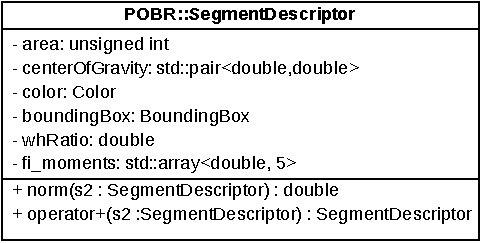
\includegraphics[width=\columnwidth]{figures/POBR-Class.pdf}
    \caption{Diagram UML klasy deskryptora segmentu}
    \label{fig:descriptor-uml}
\end{figure}

Razem z~deskryptorem, zdefiniowane zostały dwie operacje: dodawania segmentów oraz obliczania normy różnicy dwóch segmentów. Dodawanie segmentów polega na złączeniu dwóch list punktów oraz ponownym obliczeniu cech segmentów, natomiast obliczanie normy różnicy dwóch segmentów sprowadza się do policzenia sumy kwadratów różnic pomiędzy poszczególnymi momentami niezmienniczymi $\phi_{i}$, czyli odległości euklidesowskiej w~przestrzeni rozpiętej przez te momenty.

\subsubsection{Inne możliwe podejścia}
Przedstawiony powyżej sposób nie jest oczywiście jedynym możliwym. Inne podejście zakłada wykorzystanie deskryptorów tekstur. Żeby uzyskać liczbowy opis tekstury w~postaci wektora cech można posłużyć się:
\begin{itemize}
    \item metodami statystycznymi opartymi na histogramach kolorów, mierzącymi kontrast, granularność, gładkość i~chropowatość obszaru,
    \item metodami spektralnymi opartymi o~pomiary autokorelacji i~parametry obrazów przefiltrowanych częstotliwościowo,
    \item metodami strukturalnymi opartymi o~badanie struktury obszaru, kolor czy wektory ruchu~\cite{perm:wyklad}.
\end{itemize} 

Do badania tekstur można wykorzystać takie narzędzia jak macierz współwystępowania Haralicka czy filtry Gabora. 

Innym podejściem jest odrzucenie jawnych deskryptorów opisujących cechy obrazu i~zastosowanie uczenia maszynowego do automatycznego wykrywania cech. Najlepszym tego typu narzędziem jest splotowa sieć neuronowa. Każda warstwa splotowa przyjmuje na wejściu obraz lub mapę cech niższego poziomu i~tworzy nowy zbiór nowych map cech. Wyższe warstwy sieci splotowej agregują większe obszary obrazu. 

Uzyskane zbiory filtrów i~cech są optymalizowane względem konkretnego zestawu danych uczących, dlatego niekoniecznie muszą być łatwe w~ludzkiej iterpretacji~\cite{perm:wyklad}.

\section{Identyfikacja}
\label{sec:identyfikacja-cech}
Ostatnim krokiem algorytmu wykrywania logo \bk jest identyfikacja obszarów. Zadaniem identyfikacji jest stwierdzenie na podstawie otrzymanego opisu kształtu, jakiego obiektu jest on obrazem. Zasadniczo, wyróżnia się dwa podejścia: klasyfikację w~przestrzeni cech oraz klasyfikację strukturalną~\cite{pobr:wyklad}.

Klasyfikacja w~przestrzeni cech polega na porównaniu wektorów policzonych wcześniej cech. Głównym założeniem tego podejścia jest fakt, że punkty w~przestrzeni cech odpowiadające obrazom tych samych obiektów, leżą blisko siebie. Klasyfikacja czy dany segment jest obrazem danego obiektu sprowadza się do policzenia odległości dwóch punktów w~przestrzeni cech i~porównaniu jej z~danym progiem wiarygodności. Im większy próg wiarygodności, tym więcej obiektów system będzie w~stanie wyłapać, przepuszczając przy tym segmenty które nie są danym obiektem (odczyt fałszywie pozytywny). Zmniejszając próg, zwiększymy dokładność systemu kosztem większej ilości odrzuconych poprawnych segmentów (odczytów fałszywie negatywnych).

Drugim podejściem jest klasyfikacja strukturalna. Służy ona do identyfikacji złożonych obiektów. Opiera się o~analizę relacji pomiędzy obiektami składowymi, identyfikowanego obietku~\cite{pobr:wyklad}. W~tym podejściu, obraz traktowany jest dwutorowo: jako zbiór obiektów elementarnych oraz jako zbiór relacji zachodzących pomiędzy nimi.

\subsubsection{Realizacja w projekcie}
W~zadaniu projektowym posłużyłem się metodą mieszaną, korzystającą z~obu podejść. W~pierwszej kolejności segmenty były grupowane ze względu na kolor, a~następnie porównywane ze wzorcem kształtu. Wzorce zostały wyznaczone w~sposób eksperymentalny, poprzez badanie wartości momentów dla obrazów wzorcowych. Dla każdej badanej cechy, wyznaczona została średnia estymata cechy -- mediana. Zdecydowałem się na wykorzystanie mediany, ponieważ jest ona mniej obciążonym estymatorem od średniej arytmetycznej (mniej reaguje na wartości odstające). Oprócz mediany, obliczone zostało odchylenie standardowe, które miało posłużyć do wyznaczenia przedziałów wiarygodności. 

Modele zostały osobno wyznaczone dla:
\begin{itemize}
    \item białego okrągłego tła,
    \item niebieskiego paska okalającego napis,
    \item żółtej górnej bułki,
    \item żółtej dolnej bułki. 
\end{itemize}

Zdecydowałem się na pominięcie czerwonych liter w~znaku, ponieważ po przeprowadzonej segmetacji, litery często zlewały się w~jeden segment, uniemożliwiając przy tym wykrywanie pojedynczych znaków. 

W pierwszym kroku, segmenty były dzielone na grupy ze względu na ich kolor, a~następnie dla segmentów białych, niebieskich i~żółtych sprawdzano ich kształty, poprzez porównanie momentów niezmienniczych z~podanym modelem. Jeżeli suma różnic kwadratów mieściła się w~danym przedziale, przeprowadzany był kolejny test, sprawdzający zgodność współczynnika szerokości do wysokości segmentu. Jeżeli dany segment przeszedł oba testy, był on przekazywany do dalszej analizy jako potencjalny element wykrytego loga.

Po przeprowadzeniu identyfikacji obiektów bazowych w~przestrzeni cech, przyszedł czas na identyfikację strukturalną. Odbywała się ona w~trzech etapach:

\begin{itemize}
    \item znalezienie par zółtych bułek,
    \item dopasowanie białego tła dla każdej pary,
    \item potwierdzenie przez dobranie szczegółów (czerwonych liter i~niebieskiego paska).
\end{itemize}

W~pierwszym kroku, każdy z~żółtych segmentów był dobierany w~pary i~sprawdzana była odległość między nimi oraz ich porównywane były ich stosunki szerokości do wysokości.
W~wyniku analizy danych, udało mi się stwierdzić że jeżeli segmenty rzeczywiście były elementami jednego logo to odległość pomiędzy ich środkami ciężkości $d_{ij}$ nie przekraczała ona wysokości większej z~bułek więcej niż $3{,}5$ raza. Co więcej, stosunek stosunków szerokości do wysokości mieścił się w~przedziale $[0{,}8;1{,}3]$.

\begin{equation}
    \begin{aligned}
        d_{ij} &= 3{,}5 * max(h_{i}, h_{j}) \\
        0{,}8 &\leq \frac{r^{wh}_{i}}{r^{wh}_{j}} \leq 1{,}3 \\
    \end{aligned}
    \label{eqn:buns}
\end{equation}

Wszystkie pary które spełniają oba warunki są łączone w~jeden, nowy deskryptor segmentu.

Kolejnym etapem jest dopasowanie białego tła do każdej pary bułek. W~tym celu dla każdej pary, sprawdzana jest zgodność z~każdym białym segmentem. Segmenty są zgodne jeżeli środek ciężkości pary bułek znajduje się w~największym prostokącie opisanym na segmencie tła. Taki sposób może dopasowywanie z~tłem może dać wyniki z~wieloma białymi segmentami, dlatego ostatecznie, do dalszej analizy przechodzi największe znalezione tło. Po tym kroku ponownie tworzony jest nowy deskryptor segmentu, składający się ze znalezionego tła oraz wcześniej wykrytej pary bułek.

W~ostatnim kroku, algorytm szuka w~poszukiwanym fragmencie obrazu, szczegółów potwierdzających że dany segment rzeczywiście jest logiem \bk. Potwierdzanie odbywa się poprzez mechanizm głosowania. Każdy czerwony segment, którego środek ciężkości znajduje się w~sprawdzanym logo dodaje do wyniku $0{,}1$ głosu. Każdy niebieski segment, który nie został odfiltrowany w~wyniki identyfikacji w~przestrzeni cech, znajdujący się w~sprawdzanym logo dodaje do wyniki $0{,}3$ głosu. Jeżeli suma głosów przekroczy założony próg ($T_{v} = 0{,}7$), to dany segment zostaje potwierdzony jako logo. Taki sposób analizy pozwala na wykrywanie wielu poszukiwanych znaków na jednym obrazie.  

\section{Podsumowanie}
\label{sec:podsumowanie}
\todo{Króciutkie podsumowanie że projekt był fajny i takie tam}

\bibliographystyle{abbrv}
\bibliography{bibliography}

\end{document}